% mainfile: ../../main.tex
\chapter{The \pyspeck software package}\label{ch:speck:software}
\AutoLettrine{In} this chapter, I introduce the \pyspeck \python package\sidenote{
    The package repository is hosted on \href{https://git.rwth-aachen.de/qutech/python-spectrometer/}{GitLab}.
    Its documentation is automatically generated and hosted on \href{https://qutech.pages.rwth-aachen.de/python-spectrometer/}{GitLab Pages}.
    Releases are automatically published to \href{https://pypi.org/project/python-spectrometer/}{PyPI} and allow the package to be installed using \code{pip install python-spectrometer}.
}~\cite{Hangleiter_pyspeck}
and lay out its design and functionality.
This software package was developed to make it easier for experimentalists to transfer the mathematical machinery introduced in \cref{ch:speck:theory} to the lab.
While in principle the entire process of spectrum estimation from a given array of time series data is already covered by the \code{welch()} routine in \scipy~\cite{WelchScipy}, obtaining the data array is not standardized.
Different \gls{daq} instruments have different capabilities, both on the hardware and the software level, and different driver interfaces to communicate with them.
This implies that custom \acrlong{daq} code is required for every instrument, introducing a significant entry barrier to spectral analysis.
The \pyspeck package implements a simple interface to different hardware instruments that allows for changing the hardware backend without having to adapt the user-facing code and also incorporates different hardware constraints.

What is more, noise spectroscopy tends to be a visual endeavor in practice; it is hard to compare different noise spectra based on quantitative reasoning alone.
Data visualization is hence an integral part of noise spectroscopy, but plotting is not just plotting.
Do we want the data to be shown on a log-log scale?\sidenote{
    The short answer is yes, but it comes with visual side-effects that demand other ways of plotting data at times.
    The long answer is therefore yes, \emph{and} \dots
}
Do we want to show the relative magnitude of different data sets?
Do we want to inspect the time traces as well?
The \pyspeck package addresses these questions by allowing users to interactively change features of the main plot window to adapt it to the form best suited to the situation at hand.

Moreover, when concerned with noise spectrum estimation, we are typically more interested in specifying parameters of the resulting \gls{psd} rather than parameters of the underlying time series data.
The \pyspeck package approaches \acrlong{daq} from the inverse direction: rather than inferring the spectrum properties from the time series data, users specify the properties they would like the resulting spectrum to have and the package chooses the correct parameters for \acrlong{daq} accordingly.

\section{Package design and implementation}\label{sec:speck:software:design}
\begin{marginfigure}[*-10]
    \forestset{
    dir tree/.style={
        for tree={
            parent anchor=south west,
            child anchor=west,
            anchor=mid west,
            inner ysep=0pt,
            grow'=0,
            align=left,
            s sep=1ex,
            edge path={
                \noexpand\path [draw, \forestoption{edge}] (!u.parent anchor) ++(0.75em,0) |- (.child anchor)\forestoption{edge label};
            },
            font=\footnotesize\ttfamily,
            if n children=0{}{
                delay={
                    prepend={[,phantom, calign with current]}
                }
            },
            fit=band,
            before computing xy={
                l=1.5em
            }
        },
    }
}
\begin{forest}
    dir tree
    [
        [{\faIcon[regular]{folder} \pyspeckpath{doc}{doc}}]
        [{\faIcon[regular]{folder-open} \pyspeckpath{src}{src}}
            [{\faIcon[regular]{folder-open} \pyspeckpath{src/python_spectrometer}{python\_spectrometer}}
                [{\faIcon[regular]{folder-open} \pyspeckpath{src/python_spectrometer/daq}{daq}}
                    [{\faIcon[regular]{file-code} \pyspeckpath{src/python_spectrometer/daq/__init__.py}{\_\_init\_\_.py}}]
                    [{\faIcon[regular]{file-code} \pyspeckpath{src/python_spectrometer/daq/base.py}{base.py}}]
                    [{\faIcon[regular]{file-code} \pyspeckpath{src/python_spectrometer/daq/qcodes.py}{qcodes.py}}]
                    [{\faIcon[regular]{file-code} \pyspeckpath{src/python_spectrometer/daq/settings.py}{settings.py}}]
                    [{\faIcon[regular]{file-code} \ldots}]
                ]
                [{\faIcon[regular]{file-code} \pyspeckpath{src/python_spectrometer/__init__.py}{\_\_init\_\_.py}}]
                [{\faIcon[regular]{file-code} \pyspeckpath{src/python_spectrometer/_audio_manager.py}{\_audio\_manager.py}}]
                [{\faIcon[regular]{file-code} \pyspeckpath{src/python_spectrometer/_plot_manager.py}{\_plot\_manager.py}}]
                [{\faIcon[regular]{file-code} \pyspeckpath{src/python_spectrometer/core.py}{core.py}}]
            ]
        ]
        [{\faIcon[regular]{folder} \pyspeckpath{tests}{tests}}]
        [{\faIcon[regular]{file-code} \pyspeckpath{pyproject.toml}{pyproject.toml}}]
        [{\faIcon[regular]{file-code} \ldots}]
    ]
\end{forest}

    \caption[\imgsource{img/tikz/spectrometer/speck_tree.tex}]{
        Source tree structure of the \pyspeck package.
        Driver wrappers are placed in the \code{daq} subpackage.
        \code{core.py} exports the \code{Spectrometer} class.
    }
    \label{fig:speck:software:tree}
\end{marginfigure}
The \pyspeck package provides a central class, \pyinline[breakanywhere]{Spectrometer}, that users interact with to perform data acquisition, spectrum estimation, and plotting.
It is instantiated with an instance of a child class of the \code{DAQ} base class that implements an interface to various \gls{daq} hardware devices.\sidenote[][*10]{
    Actually \emph{drivers} to be more precise.
}
New spectra are obtained by calling the \code{Spectrometer.take()} method with all acquisition and metadata settings.
In the following, I will go over the the design of these aspects of the package in more detail.

\subsection{Data acquisition}\label{subsec:speck:software:design:daq}
\Cref{fig:speck:software:tree} shows the directory structure of the source code.
The \code{daq} subpackage contains on the one hand the declaration of the \code{DAQ} abstract base class (\code{base.py}) and its child class implementations (\code{qcodes.py}, \etc), and on the other the \code{settings.py} module, which defines the \code{DAQSettings} class.
This class is used in the background to validate data acquisition settings both for consistency (see \cref{sec:speck:theory:welch:parameters}) and hardware constraints.

\begin{margintable}
    \footnotesize
    \centering
    \setmintedinline[Python]{fontsize=\footnotesize}
    \caption[Overview of spectrum estimation parameters]{
        Variable names used in \cref{ch:speck:theory} and their corresponding parameter names as used in \pyspeck and \code{scipy.signal.welch()}~\cite{WelchScipy}.
    }
    \label{tab:speck:software:parameters}
    \begin{tabular}{ c C }
        \toprule
        \textsc{Variable} & \multicolumn{1}{c}{\textsc{Parameter}} \\ % multicolumn to override column type
        \midrule
        $L$ & n_pts \\
        $N$ & nperseg \\
        $K$ & noverlap \\
        $M$ & n_seg \\
        $O$ & n_avg \\
        \fs & fs \\
        \fmax & f_max \\
        \fmin & f_min \\
        \bottomrule
    \end{tabular}
\end{margintable}

To better understand the necessity of this functionality, consider the typical scenario of a physicist\sidenote{
    Let's call her Alice.
}
in the lab.
Alice has wired up her experiment, performed a first measurement, and to her dismay discovered that the data is too noisy to see the sought-after effect.
She sets up the \pyspeck code to investigate the noise spectrum of her measurement setup.
From her noisy data she could already estimate the frequency of the most harrowing noise, so she knows the frequency band $[\fmin, \fmax]$ she is most interested in.
But because she is lazy, she does not want to do the mental gymnastics to convert \fmin to the parameter that her \gls{daq} device understands, $L$ (see \cref{tab:speck:software:parameters}), especially considering that $L$ depends on the number of Welch averages and the overlap.
Furthermore, while she could just about do the conversion from \fmax to the other relevant \gls{daq} parameter, \fs, in her head, her device imposes hardware constraints on the allowed sample rates she can select!
The \code{DAQSettings} class addresses these issues.
It is instantiated with any subset of the parameters listed in \cref{tab:speck:software:parameters}\sidenote{
    \code{DAQSettings} inherits from the builtin \code{dict} and as such can contain arbitrary other keys besides those listed in \cref{tab:speck:software:parameters}.
    However, automatic validation of parameter consistency is only performed for these special keys.
}
and attempts to resolve the parameter interdependencies laid out in \cref{sec:speck:theory:welch:parameters} and depicted in \cref{fig:speck:theory:parameters} upon calling \code{DAQSettings.to_consistent_dict()}.\sidenote{
    Since the graph spanned by the parameters is not acyclic, this only works \emph{most} of the time.
}
This either infers those parameters that were not given from those that were or, if not possible, uses a default value.
Child classes of the \code{DAQ} class can subclass \code{DAQSettings} to implement hardware constraints such as a finite set of allowed sampling rates or a maximum number of samples per data buffer.

For instance, Alice might want to measure the noise spectrum in the frequency band $[\qty{1.5}{\hertz}, \qty{72}{\kilo\hertz}]$.
Although she would not have to do this explicitly,\sidenote{
    Settings are automatically parsed when passed to the \code{take()} method of the \code{Spectrometer} class.
}
she could inspect the parameters after resolution using the code shown in \cref{lst:speck:daq:settings}.

\begin{listing}[htpb]
    \begin{py}
        >>> from python_spectrometer.daq import DAQSettings
        >>> settings = DAQSettings(f_min=1.5, f_max=7.2e4)
        >>> settings.to_consistent_dict()
        {'f_min': 1.5,
         'f_max': 72000.0,
         'fs': 144000.0,
         'df': 1.5,
         'nperseg': 96000,
         'noverlap': 48000,
         'n_seg': 5,
         'n_pts': 288000,
         'n_avg': 1}
    \end{py}
    \caption{
        \code{DAQSettings} example showcasing automatic parameter resolution.
        \code{n_avg} determines the number of outer averages, \ie, the number of data buffers acquired and processed individually.
    }
    \label{lst:speck:daq:settings}
\end{listing}

\begin{marginlisting}[*-5]
    \begin{py}[fontsize=\footnotesize]
    {'f_min': 14.30511474609375,
     'f_max': 72000.0,
     'fs': 234375.0,
     'df': 14.30511474609375,
     'nperseg': 16384,
     'noverlap': 0,
     'n_seg': 1,
     'n_pts': 16384,
     'n_avg': 1}
    \end{py}
    \caption[Resolved \code{DAQSettings} for MFLI Scope]{
        Resolved settings for the same input parameters as in \cref{lst:speck:daq:settings} but for the \code{ZurichInstrumentsMFLIScope} backend with hardware constraints on \code{n_pts} and \code{fs}.
    }
    \label{lst:speck:daq:settings:mfli_scope}
\end{marginlisting}

If the instrument she'd chosen for data acquisition had been a Zurich Instruments MFLI's Scope module,\sidenote[][*7]{
    \url{https://docs.zhinst.com/labone_api_user_manual/modules/scope/index.html}
}
the same requested settings would have resolved to those shown in \cref{lst:speck:daq:settings:mfli_scope}.\sidenote[][*9]{
    And issued a warning to inform the user their requested settings could not be matched.
}
This is because the Scope module constrains $L\in[2^{12},2^{14}]$ and $\fs\in\qty{60}{\mega\hertz}\times 2^{[-16, 0]} \approx \allowbreak \lbrace \qty{915.5}{\hertz}, \allowbreak \dotsc, \allowbreak \qty{30}{\mega\hertz}, \qty{60}{\mega\hertz}\rbrace$.

As already mentioned, the \code{DAQ} base class implements a common interface for different hardware backends, allowing the \code{Spectrometer} class to be hardware-agnostic.
That is, changing the instrument that is used to acquire the data does not necessitate adapting the code used to interact with the \code{Spectrometer}.
To enable this, different instruments require small wrapper drivers that map the functionality of their actual driver onto the interface dictated by the \code{DAQ} class.
This is achieved by subclassing \code{DAQ} and implementing the \code{DAQ.setup()} and \code{DAQ.acquire()} methods.
Their functionality is best illustrated by the internal workflow as representatively shown in \cref{lst:speck:daq:workflow}.

\begin{listing}[htpb]
    \begin{py}
        daq = MyDAQ(driver_handle)

        parsed_settings = daq.setup(**user_settings)
        acquisition_generator = daq.acquire(**parsed_settings)

        for data_buffer in acquisition_generator:
            estimate_psd(data_buffer)

        # Finalize, clean up, return to user code
        ...
    \end{py}
    \caption[\gls{daq} workflow pseudocode]{
        \gls{daq} workflow pseudocode.
        A \code{MyDAQ} object (representing the instrument \code{My}) is instantiated with a driver object (for instance a \href{https://github.com/microsoft/qcodes}{\qcodes} \code{Instrument}).
        The instrument is configured with the given \code{user_settings}.
        Calling the generator function \code{daq.acquire()} with the actual device settings returns a generator, iterating over which yields one data buffer per iteration.
        The data buffers can then be passed to further processing functions (the \gls{psd} estimator in our example).
    }
    \label{lst:speck:daq:workflow}
\end{listing}

When acquiring a new spectrum, all settings supplied by the user are first fed into the \code{setup()} method where instrument configuration takes place.
The method returns the actual device settings,\sidenote{
    Which might differ from the requested settings as outlined above.
}
which are then forwarded to the \code{acquire()} generator function.
Here, the instrument is armed (if necessary), and subsequently data is fetched from the device and yielded to the caller \code{n_avg} times, where \code{n_avg} is the number of outer averages.\sidenote{
    \Ie, the number of time series data batches acquired, as opposed to the number of Welch averages \code{n_seg} within one batch.
}
An exemplary implementation of a \code{DAQ} subclass for a fictitious instrument is shown in \cref{lst:speck:daq:pseudocode}.
In addition to the methods to configure the instrument and perform data acquisition, it is possible to override the \code{DAQSettings} property to implement instrument-specific hardware constraints such as, in this example, the number of samples per buffer being constrained to the discrete interval $[1, 2048]$.
Leveraging the \code{qutil.domains} module~\cite{Hangleiter_qutil}, more complex constraints such as sample rates restricted to an internal clock rate divided by a power of two\sidenote{
    See for example the implementation of the \href{https://git.rwth-aachen.de/qutech/python-spectrometer/-/blob/main/src/python_spectrometer/daq/atsaverage.py}{AlazarTech ATS9440} digitizer card.
}
can be specified.

\begin{listing}
    \begin{py}
        # daq/mydaq.py
        import dataclasses
        from qutil.domains import DiscreteInterval
        from .base import DAQ
        from .settings import DAQSettings

        @dataclasses.dataclass
        class MyDAQ(DAQ):
            handle: mydriver.DeviceHandle

            @property
            def DAQSettings(self) -> type[DAQSettings]:
                class MyDAQSettings(DAQSettings):
                    ALLOWED_NPERSEG = DiscreteInterval(1, 2048)
                return MyDAQSettings

            def setup(self, **settings) -> dict:
                settings = self.DAQSettings(settings)
                parsed_settings = settings.to_consistent_dict()
                self.handle.configure(parsed_settings)
                return parsed_settings

            def acquire(self, n_avg: int, *, **settings) -> Generator:
                self.handle.arm(n_avg)
                for _ in range(n_avg):
                    self.handle.wait_for_trigger()
                    yield self.handle.fetch()
                return self.handle.metadata
    \end{py}
    \caption[\code{DAQ} pseudocode]{
        Exemplary code for a \code{DAQ} implementation of some instrument with given driver class \code{DeviceHandle} in the package \code{mydriver}.
        The \code{MyDAQ} class is instantiated with a \code{DeviceHandle} instance.
        Optionally, the \code{DAQSettings} property can be overridden to implement hardware constraints or default values for data acquisition parameters.
        For this, the \code{qutil.domains} module provides several classes that represent bounded domains and sets.
        The \code{setup()} method parses the given acquisition settings and configures the instrument through the external driver interface \code{handle.configure()}.
        The \code{acquire()} method arms the instrument (if necessary) and loops over the number of outer averages, \code{n_avg}.
        In the body of the loop, it can wait for external triggers (or send software triggers) before yielding a batch of data fetched from the external driver interface.
        Once acquisition is done, the method can return arbitrary metadata to the \code{Spectrometer} object to attach to the stored data.
    }
    \label{lst:speck:daq:pseudocode}
\end{listing}

\subsection{Data processing}\label{subsec:speck:software:design:processing}
Once time series data has been acquired using a given \code{DAQ} backend, it could in principle immediately be used to estimate the \gls{psd} following \cref{eq:speck:psd:bartlett}.
However, it is often desirable to transform, or process, the data in some fashion.
This can include simple transformations such as accounting for the gain of a \gls{tia} and convert the voltage back to a current,\sidenote{
    Although it is of course less than trivial to discriminate between current and voltage noise in a \gls{tia}.
}
or more complex ones such as applying calibrations.
In particular, since the process of computing the \gls{psd} already involves Fourier transformation, the processing can also be performed in frequency space.

In \pyspeck, this can be done using a \code{procfn} (in the time domain) or \code{fourier_procfn} (in the Fourier domain).
The former is specified as an argument directly to the \code{Spectrometer} constructor.
It is a callable with signature \code{(x, **kwargs) -> xp}, taking as arguments the time series data and arbitrary settings passed through from the \code{take()} method, and returns the processed data.
\Cref{lst:speck:procfn} shows a simple function that accounts for the gain of an amplifier.
The latter is specified in the \code{psd_estimator} argument of the \code{Spectrometer} constructor.
This argument allows the user to specify a custom estimator for the \gls{psd}, in which case a callable is expected.
Otherwise, it should be a mapping containing parameters for the default \gls{psd} estimator, \code{scipy.signal.welch()}~\cite{WelchScipy}.
Here, the keyword \code{fourier_procfn} should be a callable with signature \code{(xf, f, **kwargs) -> (xfp, fp)}.\sidenote{
    \Ie, the \code{psd_estimator} argument would be \code{{"fourier_procfn": fn}}.
}
That is, it should take the frequency-space data, the corresponding frequencies, and arbitrary keyword arguments and return a tuple of the processed data and the corresponding frequencies.

\begin{marginlisting}[*2]
    \begin{py}[fontsize=\footnotesize]
        def comp_gain(x, gain=1.0, **_):
            return x / gain
    \end{py}
    \caption[Simple \code{procfn} example]{
        A simple \code{procfn}, which converts amplified data back to the level before amplification.
        Note the token \code{**_} variable keyword argument that ensures no errors arise from other parameters being passed to the function.
        More complex processing chains can concisely be defined with \code{qutil.functools.FunctionChain} that pipes the output of one function into the input of the next.
    }
    \label{lst:speck:procfn}
\end{marginlisting}

A simple example for a processing function in Fourier space is shown in \cref{lst:speck:fourier_procfn}, which computes the \mbox{(anti-)}derivative of the data using the fact that
\begin{align}\label{eq:speck:fourier_derivative}
    \pdv[n]{t} \xrightarrow{\mathrm{F.T.}} \left(\i\omega\right)^n
\end{align}
under the Fourier transform.
In \cref{sec:setup:vibrations:optic}, I discuss more complex use-cases of the processing functionality included in \pyspeck in the context of vibration spectroscopy.

\begin{marginlisting}[*4]
    \begin{py}[fontsize=\footnotesize]
        def derivative(xf, f, n=0, **_):
            return xf / (2j * pi * f)**n
    \end{py}
    \caption[Simple \code{fourier_procfn} example]{A simple \code{fourier_procfn}, which calculates the \mbox{(anti-)}derivative.}
    \label{lst:speck:fourier_procfn}
\end{marginlisting}

\section{Feature overview}\label{sec:speck:software:features}
Now that we have a basic understanding of the design choices underlying \pyspeck, let us discuss the typical workflow of using the package.
Two modes of operation are to be distinguished: first, \enquote{serial} mode, in which users record new spectra manually, and second, \enquote{live} mode, in which new data is continuously being acquired.
The former is well suited to a structured approach to noise spectroscopy where data is retained persistently and discrete changes are made to the system in between subsequent data acquisitions.
The latter is aimed at a more fluent workflow in which data is not retained and data acquisition runs in the background.

\subsection{Serial spectrum acquisition}\label{subsec:speck:software:features:serial}
The default mode for spectrum acquisition using \pyspeck revolves around the \code{take()} method.
Key to this workflow is the idea that each acquired spectrum be assigned a comment that allows to easily identify it in the main plot.
For instance, this comment could contain information about the particular settings that were active when the spectrum was recorded, or where a particular cable was placed.

Consider as an example the procedure of \enquote{noise hunting}, \ie, debugging a noisy experimental setup.
The experimentalist,\sidenote{
    Let's call him Bob.
}
having discovered that his data are noisier than expected, sets up the \code{Spectrometer} class with an instance of the \code{DAQ} subclass for the \gls{daq} instrument connected to his sample, a Zurich Instruments MFLI.\sidenote{
    For the MFLI, \code{DAQ} subclasses for both the \href{https://docs.zhinst.com/labone_api_user_manual/modules/scope/index.html}{Scope} and the \href{https://docs.zhinst.com/labone_api_user_manual/modules/daq/index.html}{DAQ} module are implemented.
    The former gives access to the signal before and the latter to the signal after demodulation.
}
Choosing to work with the demodulated data to benefit from the corresponding \acrshort{daq} module's larger flexibility, he recognizes that the resulting \gls{psd} will be the two-sided version because the data returned by the \gls{lia} is complex.
Since he is interested in the physical frequencies\sidenote{
    A discussion of lock-in amplification is beyond the scope of this chapter.
    Here I will simply note that, for finite modulation frequencies $f_m$, \glspl{lia} will measure the \gls{psd} in the up-converted frequency band $[-\fmax + f_m, f_m + \fmax]$ rather than the baseband.
}
he sets the lock-in's modulation frequency to \qty{0}{\hertz} and disables plotting the negative part of the frequency spectrum as it contains only redundant data in this case.
Selecting the frequency bounds, say $\fmin = \qty{10}{\hertz}$ and $\fmax = \qty{100}{\kilo\hertz}$, and using the sensible defaults for the remaining spectrum parameters, Bob first grounds the input of his \gls{daq} to record a \emph{baseline} spectrum.
Thus far, his code would hence look something like that shown in \cref{lst:speck:workflow:serial}, which produces the plot shown in \cref{fig:speck:software:workflow:baseline}.

\begin{listing}[htpb]
    \begin{py}
        from python_spectrometer import Spectrometer, daq
        from qutil.functools import scaled

        mfli_daq = daq.ZurichInstrumentsMFLIDAQ(session, device)
        spect = Spectrometer(mfli_daq, procfn=scaled(1e6),
                             plot_negative_frequencies=False,
                             processed_unit='μV')

        settings = {'f_min': 1e1, 'f_max': 1e5, 'freq': 0}
        spect.take('baseline', daq='grounded', **settings)
    \end{py}
    \caption[\pyspeck serial workflow]{
        Setup and serial workflow using the \pyspeck package.
        \code{session} and \code{device} are \gls{api} objects of the \code{zhinst.toolkit} driver package.
        It is therefore possible to simply use the driver objects that are already in use in the measurement setup.
        The \code{procfn} and \code{processed_unit} arguments help converting raw data into a more human-friendly unit.
    }
    \label{lst:speck:workflow:serial}
\end{listing}
\begin{figure}
    \centering
    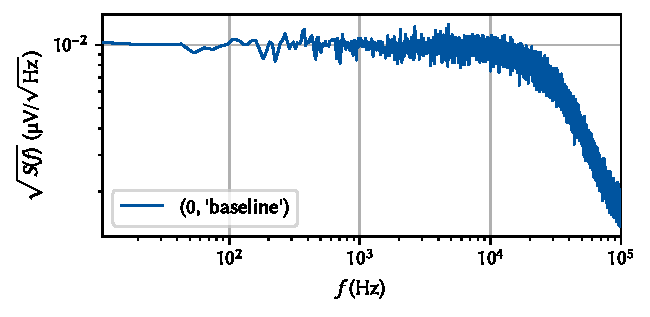
\includegraphics{img/pdf/spectrometer/workflow_baseline}
    \caption[\imgsource{img/py/spectrometer/pyspeck_workflow.py}]{
        The \pyspeck plot after acquiring the (here: synthetic) baseline spectrum.
        By default, the \gls{asd} = √\gls{psd} is displayed in the main plot.
        Each spectrum is assigned a unique identifier key consisting of an incrementing integer and the user comment, and can be referred to by either (or both) when interacting with the object.
    }
    \label{fig:speck:software:workflow:baseline}
\end{figure}

The noise spectrum he obtains is white up until approximately \qty{20}{\kilo\hertz} where it starts falling off $\propto f^{-n}$.
This is because the \gls{lia} low-pass filters the signal to suppress aliasing.\sidenote[][*-4]{
    Aliasing effects arise from finite sampling according to the Nyquist-Shannon sampling theorem~\cite{Whittaker1915,Nyquist1928,Shannon1949}.
    It states that for a given physical bandwidth, the sampling rate \fs must be at least twice as large to faithfully reconstruct the signal in order to avoid aliasing, \ie, the reverse of the argument we have made for the largest resolvable frequency \fmax.
    Some \gls{daq} devices perform internal aliasing rejection while others do not.
}
After acquiring the baseline, he next ungrounds the \gls{daq} to obtain a representative spectrum of the noise in an actual measurement.
He then proceeds by tweaking things on his setup, testing out different parameters, \etc
Every time he changes something, he acquires another spectrum using \code{take()}, labeling each with a meaningful comment for identification.
\begin{figure}
    \centering
    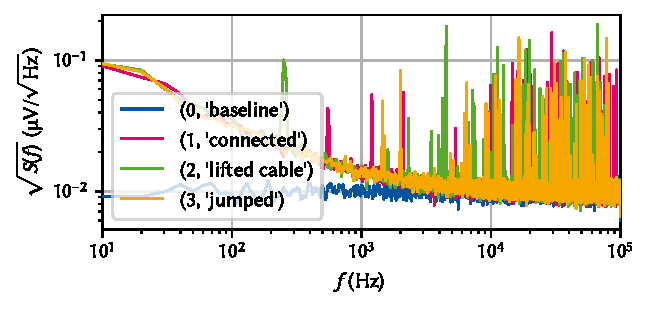
\includegraphics{img/pdf/spectrometer/workflow_spectra}
    \caption[\imgsource{img/py/spectrometer/pyspeck_workflow.py}]{
        The \pyspeck plot after acquiring additional (synthetic) spectra.
        Each spectrum is uniquely identified by a two-tuple of \code{(index, comment)}.
    }
    \label{fig:speck:software:workflow:spectra}
\end{figure}
The code shown in \cref{lst:speck:workflow:spectra} would then leave him with the spectrometer plot as shown in \cref{fig:speck:software:workflow:spectra}.
While working, Bob realizes he'd like see the signal in the time domain as well.
He easily achieves this by setting \code{spect.plot_timetrace = True}, which adds an oscilloscope subplot to the spectrometer figure as shown in \cref{fig:speck:software:workflow:timetrace}.
Since his \gls{daq} returns complex data, the absolute value $R = X + \i Y$ is plotted.

\begin{listing}[htpb]
    \begin{py}
        settings['daq'] = 'connected'
        spect.take('connected', **settings)
        spect.take('lifted cable', cable='lifted', **settings)
        spect.take('jumped', **settings)
    \end{py}
    \caption[]{
        Code to acquire additional spectra.
        Arbitrary key-value pairs can be passed to the \code{take()} method, which are stored as metadata if they do not apply to any functions downstream in the data processing chain.
    }
    \label{lst:speck:workflow:spectra}
\end{listing}
\begin{figure}
    \centering
    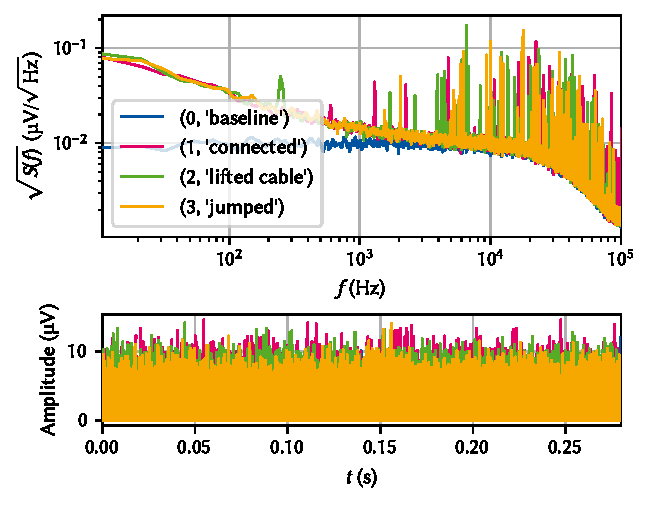
\includegraphics{img/pdf/spectrometer/workflow_timetrace}
    \caption[\imgsource{img/py/spectrometer/pyspeck_workflow.py}]{
        The \pyspeck plot shown in \cref{fig:speck:software:workflow:spectra} when setting \code{spect.plot_timetrace = True}.
        This adds a subplot that shows the time series data from which the \gls{psd} was computed akin to what an oscilloscope would show.
        For complex time series, the absolute value $R = X + \i Y$ is plotted.
        Note that this is the entire time series, \ie, the data of length $L$, which is (by default, using Welch's method) segmented for spectrum estimation.
    }
    \label{fig:speck:software:workflow:timetrace}
\end{figure}

Bob now observes that the noise spectra he has recorded display many sharp peaks in particular at high frequencies while the \oneoverf noise floor seems pretty consistent across different measurements.
This makes it harder for him to evaluate whether any of his changes are actually an improvement or not.
The \pyspeck package allows addressing this by plotting the integrated spectra in another subplot.
Bob's spectrometer figure after setting \code{spect.plot_cumulative = True} is shown in \cref{fig:speck:software:workflow:cumulative}.
In the case that \code{spect.plot_amplitude == True}, this new subplot shows the \gls{rms} in the band $[\fmin, f]$,
\begin{align}\label{eq:speck:software:cumulative}
    \rms_S(f)\equiv\rms_S(\fmin, f),
\end{align}
and the band power (\cref{eq:speck:psd:bandpower}) otherwise.

\begin{figure}
    \centering
    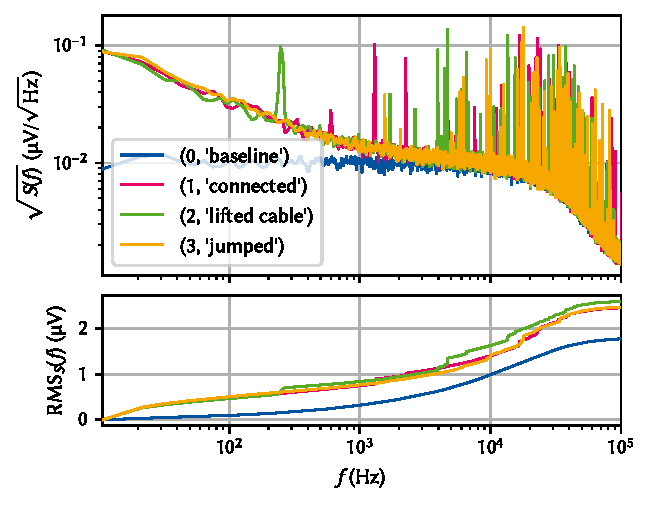
\includegraphics{img/pdf/spectrometer/workflow_cumulative}
    \caption[\imgsource{img/py/spectrometer/pyspeck_workflow.py}]{
        The \pyspeck plot shown in \cref{fig:speck:software:workflow:spectra} when setting \code{spect.plot_cumulative = True}.
        This adds a subplot that shows the \gls{rms} (see \cref{eq:speck:psd:bandpower}) which can be helpful in evaluating the contribution of individual peaks in the spectrum to the total noise power.
        Both the oscilloscope subplot (\cref{fig:speck:software:workflow:timetrace}) and the \gls{rms} subplot can also be shown at the same time.
    }
    \label{fig:speck:software:workflow:cumulative}
\end{figure}

The cumulative \gls{rms} plot already helps, but Bob would like a more quantitative comparison of relative spectral powers.
Therefore, he rescales the spectra in terms of their relative powers expressed in \unit{\decibel}\sidenote[][*-3]{
    Recall that the decibel is defined by the ratio $L_P$ of two powers $P_1, P_2$ as~\cite{Pozar2012}
    \begin{align*}
        L_P = 10\log_{10}\left(\frac{P_1}{P_2}\right)\,\unit{\decibel}.
    \end{align*}
}
by applying the following settings, which changes the plot to the layout shown in \cref{fig:speck:software:workflow:db}:

\begin{py}
    spect.plot_dB_scale = True
    spect.plot_amplitude = False
    spect.plot_density = False
\end{py}

\begin{figure}
    \centering
    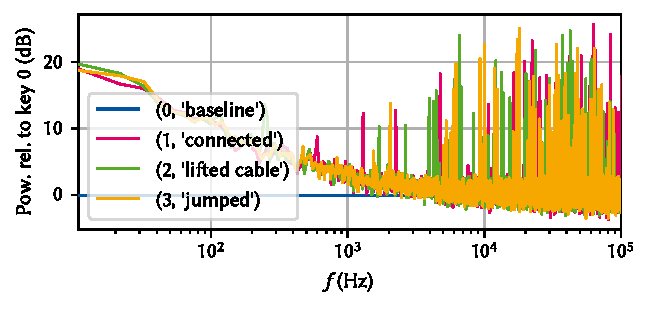
\includegraphics{img/pdf/spectrometer/workflow_db}
    \caption[\imgsource{img/py/spectrometer/pyspeck_workflow.py}]{
        The \pyspeck plot in relative mode.
        Starting from the state in \cref{fig:speck:software:workflow:spectra}, we set \code{spect.plot_dB_scale = True} as well as \code{spect.plot_amplitude = False} and \code{spect.plot_density = False} to compare the relative noise powers with respect to the baseline.
    }
    \label{fig:speck:software:workflow:db}
\end{figure}
The attribute \code{plot_density} controls whether the \emph{\acrlong{psd}} or the \emph{power spectrum} is plotted.\sidenote[][*-5]{
    \label{sidenote:speck:software_vocabulary}
    At this point, we \emph{do} need to distinguish between the \gls{psd} and the power spectrum counter to \cref{sidenote:speck:theory_vocabulary} in \cref{ch:speck:theory}.
    The \gls{psd} and power spectrum are related by the \gls{enbw},
    \begin{align*}
        \text{Spectral density} \xrightarrow{\times\enbw} \text{Spectrum},
    \end{align*}
    which is itself a function of the sampling rate and the properties of the spectral window~\cite{Harris1978},
    \begin{align}\label{eq:speck:software:enbw}
        \enbw = \fs\frac{\sum_n\hat{w}_n^2}{\left[\sum_n\hat{w}_n\right]^2}.
    \end{align}
}
Scaling the data to the power spectrum instead of the density, Bob can get an estimate of the \gls{rms} at a single frequency by reading off the peak height.
Additionally displaying the data in \unit{\decibel} then gives insight into relative noise powers of different spectra.

Bob carries on with his enterprise and continues to acquire spectra until, finally, he finds the source of his noise!
Alas, his spectrometer plot is now overflowing with plotted data when really he just wants to compare the baseline, the original, noisy state, and the final, clean spectrum.
He simply calls

\begin{py}
    spect.hide(*range(2, 10))
\end{py}

to hide the eight spectra of unsuccessful debugging, leaving him with a plot as shown in \cref{fig:speck:software:workflow:success}.

\begin{figure}
    \centering
    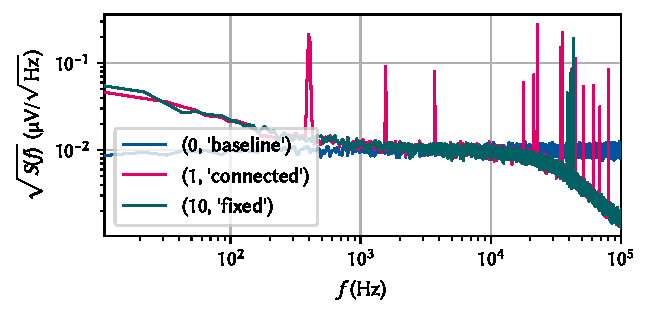
\includegraphics{img/pdf/spectrometer/workflow_success}
    \caption[\imgsource{img/py/spectrometer/pyspeck_workflow.py}]{
        The \pyspeck plot after multiple additional spectra were acquired and hidden.
        Hiding spectra that one is not interested in anymore is achieved through \code{spect.hide(*range(2, 10))}.
        This is reversed by \code{spect.show(*range(2, 10))}.
        Data can also be dropped (\code{spect.drop(key)}) or deleted (\code{spect.delete(key)}) from the internal cache and disk, respectively.
    }
    \label{fig:speck:software:workflow:success}
\end{figure}

Finally, happy with the results, Bob serializes the state of the spectrometer to disk, allowing him to pick up where he left off at a later point in time:

\begin{py}
    spect.serialize_to_disk('2032-12-24_noise_hunting')
\end{py}

The next week, Bob is asked by his team about his progress on debugging the noise in their setup.
Even though he is working from home that day and does not have access to the lab computer, Bob simply uses his laptop computer and pulls up the \code{Spectrometer} session stored on the server, allowing them to interactively discuss the spectra:

\begin{py}
    file = '2032-12-24_noise_hunting'
    # Read-only instance because no DAQ attached
    spect = Spectrometer.recall_from_disk(savepath / file)
\end{py}

This opens up the plot shown in \cref{fig:speck:software:workflow:success} again.
While they cannot acquire new spectra in this state,\sidenote{
    They could of course always attach a \code{DAQ} instance to the spectrometer and continue as they were.
}
they can still use all the plotting features like showing or hiding spectra, or changing plot types as discussed above.

\subsection{Live spectrum acquisition}\label{subsec:speck:software:features:live_view}
Manually recording spectra in the workflow outlined in \cref{subsec:speck:software:features:serial} becomes tedious at some point, and experimenters tend to become negligent with keeping metadata and comments up to date as they continue to change settings.
Once a certain number of spectra has been obtained, the spectrometer plot also becomes crowded, and hiding old spectra manually is cumbersome.
Moreover, each time a spectrum is captured, data is saved to disk, potentially accruing large amounts of storage space.
For these reasons, the \pyspeck package also offers a non-persistent live mode for displaying spectra continuously.

This mode is facilitated by the \code{qutil.plotting.live_view} module that provides asynchronous plotting functionality based on \matplotlib.
The \code{live_view} module supports both the multithreading and multiprocessing paradigms for concurrency in order to keep the interpreter responsive.\sidenote{
    Note that technically, data is also recorded in a background thread in serial mode by default.
}
In the former case, the window hosting the figure runs in the main thread and is kept responsive using \matplotlib's \gls{gui} event loop mechanisms.
In the latter, the plotting takes place in a separate process, resulting in true parallelism.

The live mode is started with the \code{Spectrometer.live_view()} method.
Data is continuously acquired in a background thread using the same \code{DAQ} interface as the serial mode.
Instead of saving the data on disk and managing plotting from \pyspeck, however, the data is fed into a queue.\sidenote{
    A queue is a concurrency mechanism for exchanging data between multiple threads or processes.
}
A \code{live_view.IncrementalLiveView2D} object then retrieves the data from the queue and handles plotting in the \gls{gui} event loop.
To start a spectroscopy session with the same parameters as in \cref{subsec:speck:software:features:serial} with a given \code{Spectrometer} object (see \cref{lst:speck:workflow:serial}), we would call

\begin{py}
    view = spect.live_view(f_min=1e1, f_max=1e5, in_process=True)
\end{py}

which would open a figure window such as that shown in \cref{fig:speck:software:live_view}.
Similar to \code{take()}, the data acquisition parameters are passed to \code{live_view()} as keyword arguments.\sidenote{
    The difference is, of course, that we do not need to specify a comment since no data is retained.
}
The \code{in_process} argument specifies if multiprocessing (\code{True}) or multithreading (\code{False}) is used.
Dictionaries with customization parameters for the \code{live_view} object can further be passed to the method.
Functionality to take snapshots to retain live data is currently not implemented but would be a valuable addition to the noise-hunting workflow.

\begin{figure}
    \centering
    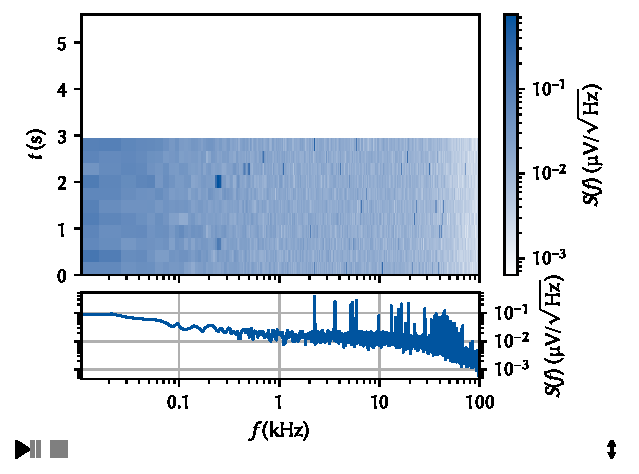
\includegraphics{img/pdf/spectrometer/live_view}
    \caption[\imgsource{img/py/spectrometer/pyspeck_live_view.py}]{
        Spectrometer live view.
        The bottom plot shows the most recently acquired spectrum, while the top plot shows a waterfall plot of the most recent ones.
        Data acquisition runs in a background thread, keeping the interpreter responsive and available to interact with instruments, for example.
        The icons in the bottom left and right corners allow interacting with the live view.
    }
    \label{fig:speck:software:live_view}
\end{figure}
